\documentclass[10pt,conference,compsocconf]{IEEEtran}

\usepackage{hyperref}
\usepackage{amsmath}        % math
\usepackage{graphicx}   % For figure environment


\begin{document}
\title{Machine learning applied to the Higgs boson CERN dataset}

\author{
  Luc\'{i}a Montero Sanchis, Nuno Mota Gon\c{c}alves, Matteo Yann Feo,  \\
  \textit{Department of Computer Science, EPFL Lausanne, Switzerland}
}

\maketitle

\begin{abstract}
  This report presents the results of applying least squares and logistic regression to the Higgs boson dataset for classification purposes. These methods are analyzed and compared for different polynomial basis degrees of the input data. We also consider applying principal component analysis to reduce the dimensionality of the feature space.
\end{abstract}

\section{Introduction}
	The aim of this project is to classify the data in the CERN dataset in two different classes, for finding the Higgs boson. This task will be carried out applying the machine learning methods learned during the course, together with the improvements that we have considered the most appropriate to overcome the challenges of this assignment. Some of the challenges of this classification process include parsing the missing information in the dataset, properly dealing with a large number of features and samples, and choosing the learning method that is the most suitable.

	The learning algorithms we focus on are least squares and logistic regression, being the latter the most adequate for classification. The possibility of including a regularization factor is considered in order to avoid overfitting. We expand the features by including a polynomial basis up to a certain degree, to achieve a higher accuracy in the classification. We also use Principal Component Analysis (PCA) to obtain a smaller number of linearly uncorrelated variables.

	%We start by presenting the models and methods used in section \ref{sec:models-methods}. We then include the results obtained, and discuss them in section \ref{sec:discussion}.

\section{Models and methods}
	\label{sec:models-methods}
	\subsection{Initial data parsing} % (fold)
	\label{sub:initial_data_parsing}
  	The Higgs boson dataset contains $250000$ observations and $30$ features or variables. These variables take values in different ranges. Certain features contain the value $-999$ for some of the observations, which we have considered to represent \emph{missing information}. %In some cases up to 29\% of the total observed data for a variable is missing.

  	Before applying a learning algorithm we verify that the features are standardized,  so that they are considered equally. To standardize the features we substract the mean and divide by the standard deviation. For the variables with missing information, the mean and the standard deviation are computed only over the non-missing values. Afterwards the missing values are set to $0$ so that they do not modify the scale of the variable. When standardizing the test data we used the mean and the standard deviation of the train data. This assures the same transformation to both datasets, although it should not make a big difference since the distribution of the training and test data is assumed to be the same.
	% subsection initial_data_parsing (end)

	\subsection{Polynomial basis} % (fold)
	\label{sub:polynomial_basis}
  	To improve the accuracy in the classification we increase the amount of explanatory variables by building a polynomial basis. We expand the features including the powers of each of the original variables up to a certain chosen degree. Since the newly included variables may have a different standard deviation, we normalize them to assure that their standard deviation is $1$. We also include an offset term.
	% subsection polynomial_basis (end)

	\subsection{Principal Component Analysis (PCA)} % (fold)
	\label{sub:principal_component_analysis}
  	The total number of features increases considerably for polynomial basis with a large degree. In these cases we reduce the dimensionality $d$ of the feature space using PCA.

  	As specified in \cite{smith02}, to do so we first find the covariance matrix of the features. We then compute the eigenvalues and eigenvectors. The eigenvectors form a basis for the data, and they can be sorted in order of \emph{decreasing} eigenvalue. We can then select a subset of the first $L\leq d$ eigenvectors as basis vectors. This allows to compare the results achieved by building a polynomial base with a larger degree and then reducing dimensionality by applying PCA, with the results achieved for a polynomial basis of a lower degree.
	% subsection principal_component_analysis (end)

	\subsection{Least squares and Ridge regression} % (fold)
	\label{sub:least_squares_and_ridge_regression}
  	We start classifying with least squares. Since it is possible to have overfitting, we consider the possibility of using ridge regression. However, the ridge regression method implemented penalizes the offset of the model, which might decrease the accuracy of the predictions.
	% subsection least_squares_and_ridge_regression (end)

	\subsection{Logistic regression and Regularized logistic regression} % (fold)
	\label{sub:logistic_regression_and_regularized_logistic_regression}
  	We focus on using this method, since it is more suitable for classifying. For the logistic regression with stochastic gradient descent algorithm we have first considered a constant learning rate $\lambda$, and then an adaptive one $\lambda^{(t)}$ as shown in \ref{eq:lr}, where $t$ is the iteration.

  	\begin{equation}
    	\label{eq:lr}
      	\lambda^{(t)} = \eta \cdot t ^{- \kappa}
  	\end{equation}

  	Although by using an adaptive learning rate we increase the number of hyperparameters to adjust, the convergence improves.
  	As for least squares, there is a possibility of overfitting when considering a large degree for the polynomial basis. In this case we would use regularized logistic regression, which would result into a third hyperparameter to adjust. The regularization implementation in this case does not penalize the offset term of the model, solving the problem mentioned previously.
	% subsection logistic_regression_and_regularized_logistic_regression (end)

	\subsection{Cross validation and hyperparameters tuning} % (fold)
	\label{sub:cross_validation_and_hyperparameters_tuning}
  	For the cross validation we have considered $80\%$ of the data for training and $20\%$ for test. Out of the \emph{training} data, $80\%$ is used for training and the remaning $20\%$ for validation (i.e. for tuning the hyperparameters). To compare the classification errors for each model, we define \emph{accuracy} as the ratio of correct predictions.	We choose the parameters for the adaptive learning rate $\lambda^{(t)}$ and the regularization factor $\gamma$ by using a random layout (random search).
	% subsection cross_validation_and_hyperparameters_tuning (end)

\section{Results}
\label{sec:results}
    We first predict the labels for the test data using least squares, that we implement using the normal equations. After building the polynomial basis with degrees $2$ to $8$ for the training data, we apply least squares. Figure \ref{fig:LSprec} shows the accuracy obtained for the training, validation and test data for each maximum degree.

    \begin{figure}[htp]
      \centering
      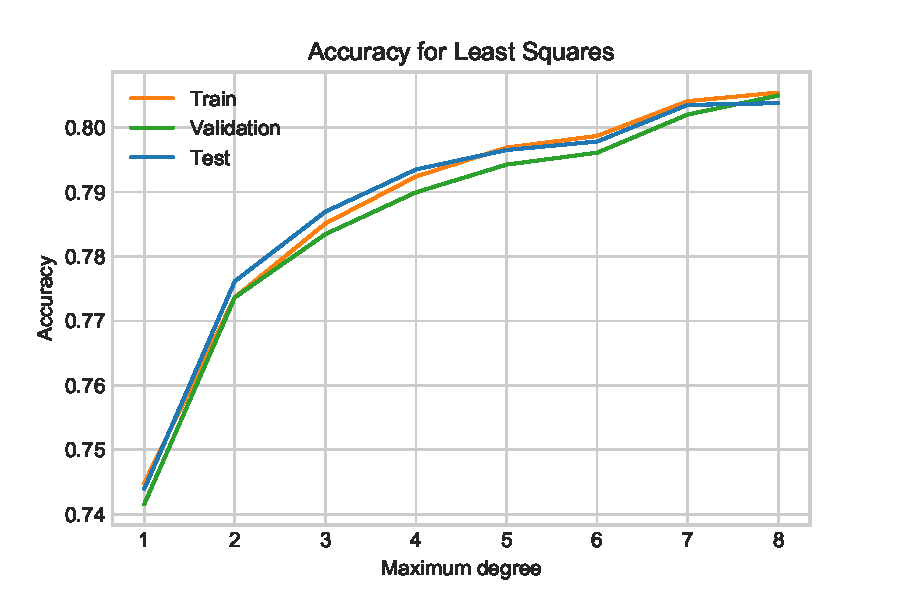
\includegraphics[width=.45\textwidth]{LSprec}
      \caption{Accuracy achieved using Least squares}
      \label{fig:LSprec}
    \end{figure}

    %\begin{figure}[htp]
      %\centering
      %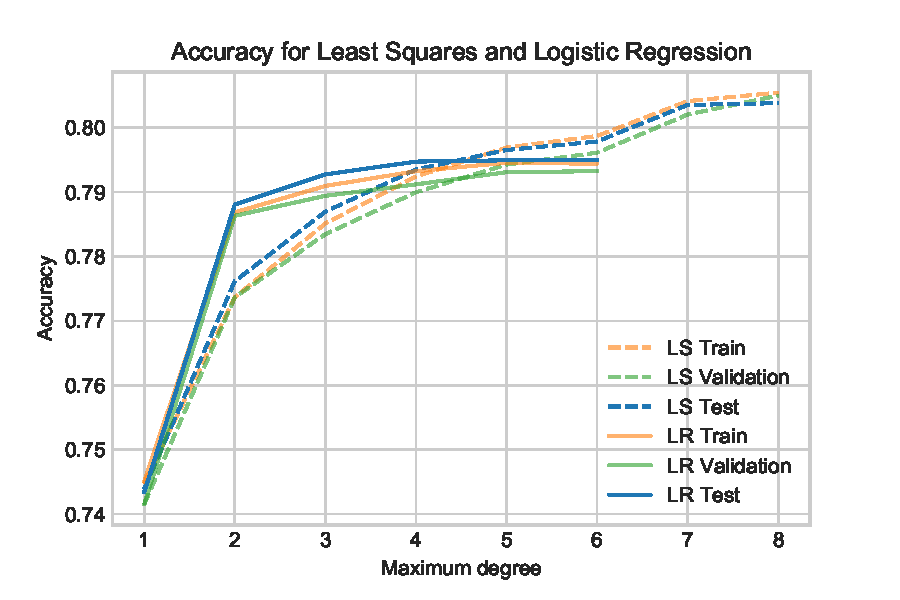
\includegraphics[width=.45\textwidth]{LSLRprec}
      %\caption{Accuracy achieved using Least squares and Logistic Regression}
      %\label{fig:LSLRprec}
    %\end{figure}

    The accuracy increases for larger maximum degrees, and the increase in accuracy with respect to the degree gets lower as the degree gets larger. We also observe that there does not seem to be an overfitting, since the difference in precision between the training and the validation-test predictions do not seem large.

    We then use the logistic regression Stochastic Gradient Descent (SGD) algorithm, with batch size $2000$ and $1500$ iterations. As explained previously, we use an adaptive learning rate that is defined by two hyperparameters. In this case, the values are $\eta = 10^{-2}$ and $\kappa = 0.8$.

    Figure \ref{fig:LRprec} shows the accuracy obtained for the training, validation and test data for each maximum degree using logistic regression.

    \begin{figure}[htp]
      \centering
      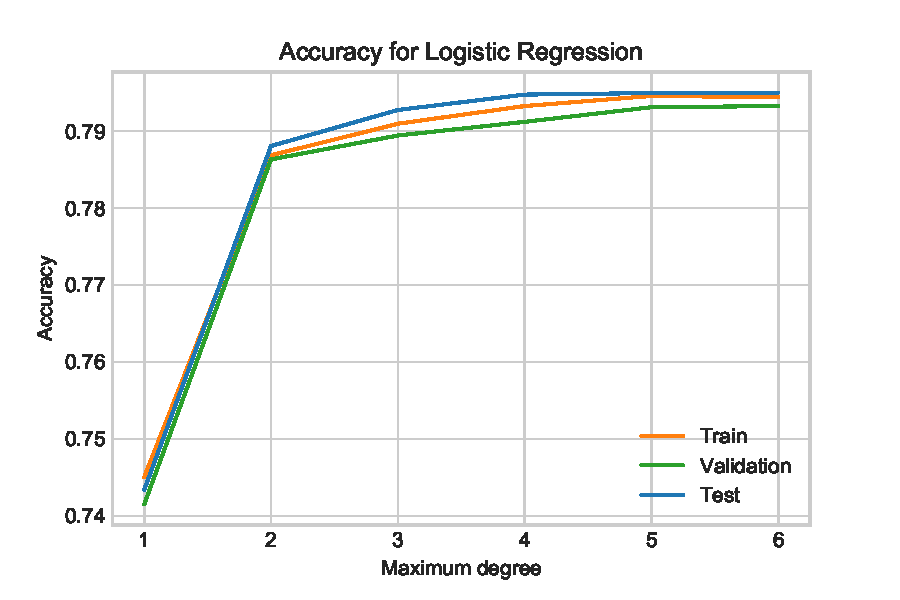
\includegraphics[width=.45\textwidth]{LRprec}
      \caption{Accuracy achieved using Logistic regression}
      \label{fig:LRprec}
    \end{figure}

    In this case we can again see that the accuracy increases with the degree of the polynomial, and that the model does not seem to overfit. Therefore, we do not include a regularization factor. As seen with least squares, the increment in accuracy is smaller for the largest degrees.

    TODOPrincipal component analysis

\section{Discussion}
\label{sec:discussion}
  In the results section we have shown that the accuracy obtained higher when considering a polynomial basis of a larger degree, since for larger degrees there are more features to consider when fitting the model. However, it has been shown as well that this difference in accuracy is larger when the degrees being compared are small. For instance, when using least squares it is not clear if it is worth it to consider a basis of degree $8$ as compared to using a basis of degree $7$. It is interesting as well to note that we did not find cases of overfitting when using either least squares or logistic regression.

  We also found that although we expected the logistic regression algorithm to perform better than least squares, both achieve a similar accuracy for a same degree of polynomial. In fact, for some degrees least squares outperforms logistic regression. A possible reason for this is that we are obtaining the analytical solution for the least squares algorithm, whereas for logistic regression we have estimated it by choosing a series of parameters (learning rate, number of iterations, and size of the batch for SGD).

  TODO: algo de PCA

\section{Summary}
\label{sec:tips-writing}
  The difference in performance for least squares and logistic regression has not been large enough for us to withdraw any final conclusions about which method is best for classification of this dataset. We have however seen that the accuracy is higher for a higher degree of the polynomial database or for a higher feature space dimension. Increasing the degree and applying PCA to reduce the number of features is not worth for the cases considered.

\bibliographystyle{IEEEtran}
\bibliography{literature}

\end{document}
